
\documentclass[twoside,12pt]{article}
%\documentclass[UTF8]{ctexart}
\usepackage[heading=true]{ctex}

\RequirePackage{natbib}
% modification to natbib citations
\setcitestyle{authoryear,round,citesep={;},aysep={,},yysep={;}}

\usepackage{listings}
\usepackage{color}

\definecolor{dkgreen}{rgb}{0,0.6,0}
\definecolor{gray}{rgb}{0.5,0.5,0.5}
\definecolor{mauve}{rgb}{0.58,0,0.82}

\lstset{frame=tb,
  language=Python,
  aboveskip=3mm,
  belowskip=3mm,
  showstringspaces=false,
  columns=flexible,
  basicstyle={\small\ttfamily},
  numbers=none,
  numberstyle=\tiny\color{gray},
  keywordstyle=\color{blue},
  commentstyle=\color{dkgreen},
  stringstyle=\color{mauve},
  breaklines=true,
  breakatwhitespace=true,
  tabsize=3
}

\usepackage{fancyhdr} % 页眉页脚
\usepackage{graphicx}
\usepackage{amsmath}
\usepackage[colorlinks=true, allcolors=blue]{hyperref}
\usepackage{geometry}

\geometry{
  paper      = a4paper,
  vmargin    = 2.54cm,
  hmargin    = 3.17cm,
  headheight = 0.75cm,
  headsep    = 0.29cm,
  footskip   = 0.79cm,
}


\newcommand{\update}[1]{{\textcolor{black}{#1}}}
\newcommand{\boldres}[1]{{\textbf{\textcolor{red}{#1}}}}
\newcommand{\secondres}[1]{{\underline{\textcolor{blue}{#1}}}}

\pagestyle{fancy}

%\firstpageno{1}

\title{ }

\author{罗浩铭\ PB21030838}


\begin{document}

\fancyhf{} % 清除所有页眉页脚
\fancyfoot[C]{\thepage} % 设置右页脚为页码
\fancyhead[l]{\footnotesize  }
% 设置右页眉为章节标题 

\renewcommand{\headrulewidth}{0pt} % 去页眉线

\begin{center}
  \textbf{\LARGE{iTransformer论文翻译报告}}\\
  \vspace{0.2cm}
  \large{罗浩铭\ PB21030838}
\end{center}

% 找一篇2021年以后的知名会议和期刊上发表的人工智能相关的文章,翻译其摘要与Introduction部分,写一篇翻译报告(附上原文与翻译后的中文)
% 文章翻译正确,流畅,通顺,信达雅

\section{文章基本信息}

\begin{itemize}
  \item 论文题目:iTransformer: Inverted Transformers Are Effective for Time Series Forecasting~\citep{itransformer}
  \item 论文作者:Yong Liu, Tengge Hu, Haoran Zhang, Haixu Wu, Shiyu Wang, Lintao Ma, Mingsheng Long
  \item 论文来源:ICLR 2024(在投,但在OpenReview已经拿到3个8分和一个6分,基本确定中会,参见https://openreview.net/forum?id=JePfAI8fah)
  \item 首发日期:2023年10月10日
  \item 论文链接:\url{https://arxiv.org/abs/2310.06625}
  \item 论文官方实现:\url{https://github.com/thuml/iTransformer}(截至本报告完成时,已获得443颗星)
\end{itemize}

\section{摘要}
\subsection{译文}
近年来,线性时间序列预测模型迅速兴起,这对此前人们一直热衷的路线——改进基于Transformer的预测模型架构——提出了质疑。这些预测器利用Transformer来将时间序列中同一时间点的所有变量值建模为temporal tokens,由此来捕捉各时间点的变量之间的全局依赖关系。然而,Transformer架构的模型在以更长的历史序列为输入时,会遭遇性能下降与计算量剧增的挑战。此外,对于每个temporal token融合的多个变量,它们可能具有不同物理意义,采集时间可能并不对齐,且尺度可能差异较大,这将使得模型无法学习到以变量为中心的表征,并使得模型学习到无意义的注意力矩阵。在这项工作中,我们重新思考了Transformer组件在整个架构中的用途和地位,并在不修改任何底层组件的情况下提出了我们的新架构。我们提出了\textbf{iTransformer},它简单地互换注意力机制和FFN作用的维度。具体来说,它将同一个变量的序列建模为variate tokens,并在此之上使用注意力机制来捕捉变量之间的联系;同时,它对各variate tokens使用FFN来获取其非线性表示。我们的iTransformer架构在各大富有挑战的真实世界数据集中都取得了SOTA的效果,增强了整个Transformer系列的性能、在不同变量间的泛化能力以及对任意输入序列长度的更好利用,这使其成为时间序列分析任务中一个强有力的backbone竞争方案。

\subsection{原文}
The recent boom of linear forecasting models questions the ongoing passion for architectural modifications of Transformer-based forecasters. These forecasters leverage Transformers to model the global dependencies over \emph{temporal tokens} of time series, with each token formed by multiple variates of the same timestamp. However, Transformers are challenged in forecasting series with larger lookback windows due to performance degradation and computation explosion. Besides, the embedding for each temporal token fuses multiple variates \update{that represent potential delayed events and distinct physical measurements}, which may fail in learning variate-centric representations and result in meaningless attention maps. In this work, we reflect on the competent duties of Transformer components and repurpose the Transformer architecture without any modification to the basic components. We propose \textbf{iTransformer} that simply \update{applies the attention and feed-forward network on the inverted dimensions}. Specifically, the time points of individual series are embedded into \emph{variate tokens} which are utilized by the attention mechanism to capture multivariate correlations; meanwhile, the feed-forward network is applied for each variate token to learn nonlinear representations. The iTransformer model achieves state-of-the-art on challenging real-world datasets, which further empowers the Transformer family with promoted performance, generalization ability across different variates, and better utilization of arbitrary lookback windows, making it a nice alternative as the fundamental backbone of time series forecasting.

\section{Introduction部分}
\subsection{译文}

\subsection{原文}

\begin{figure}[t]
  \begin{center}
    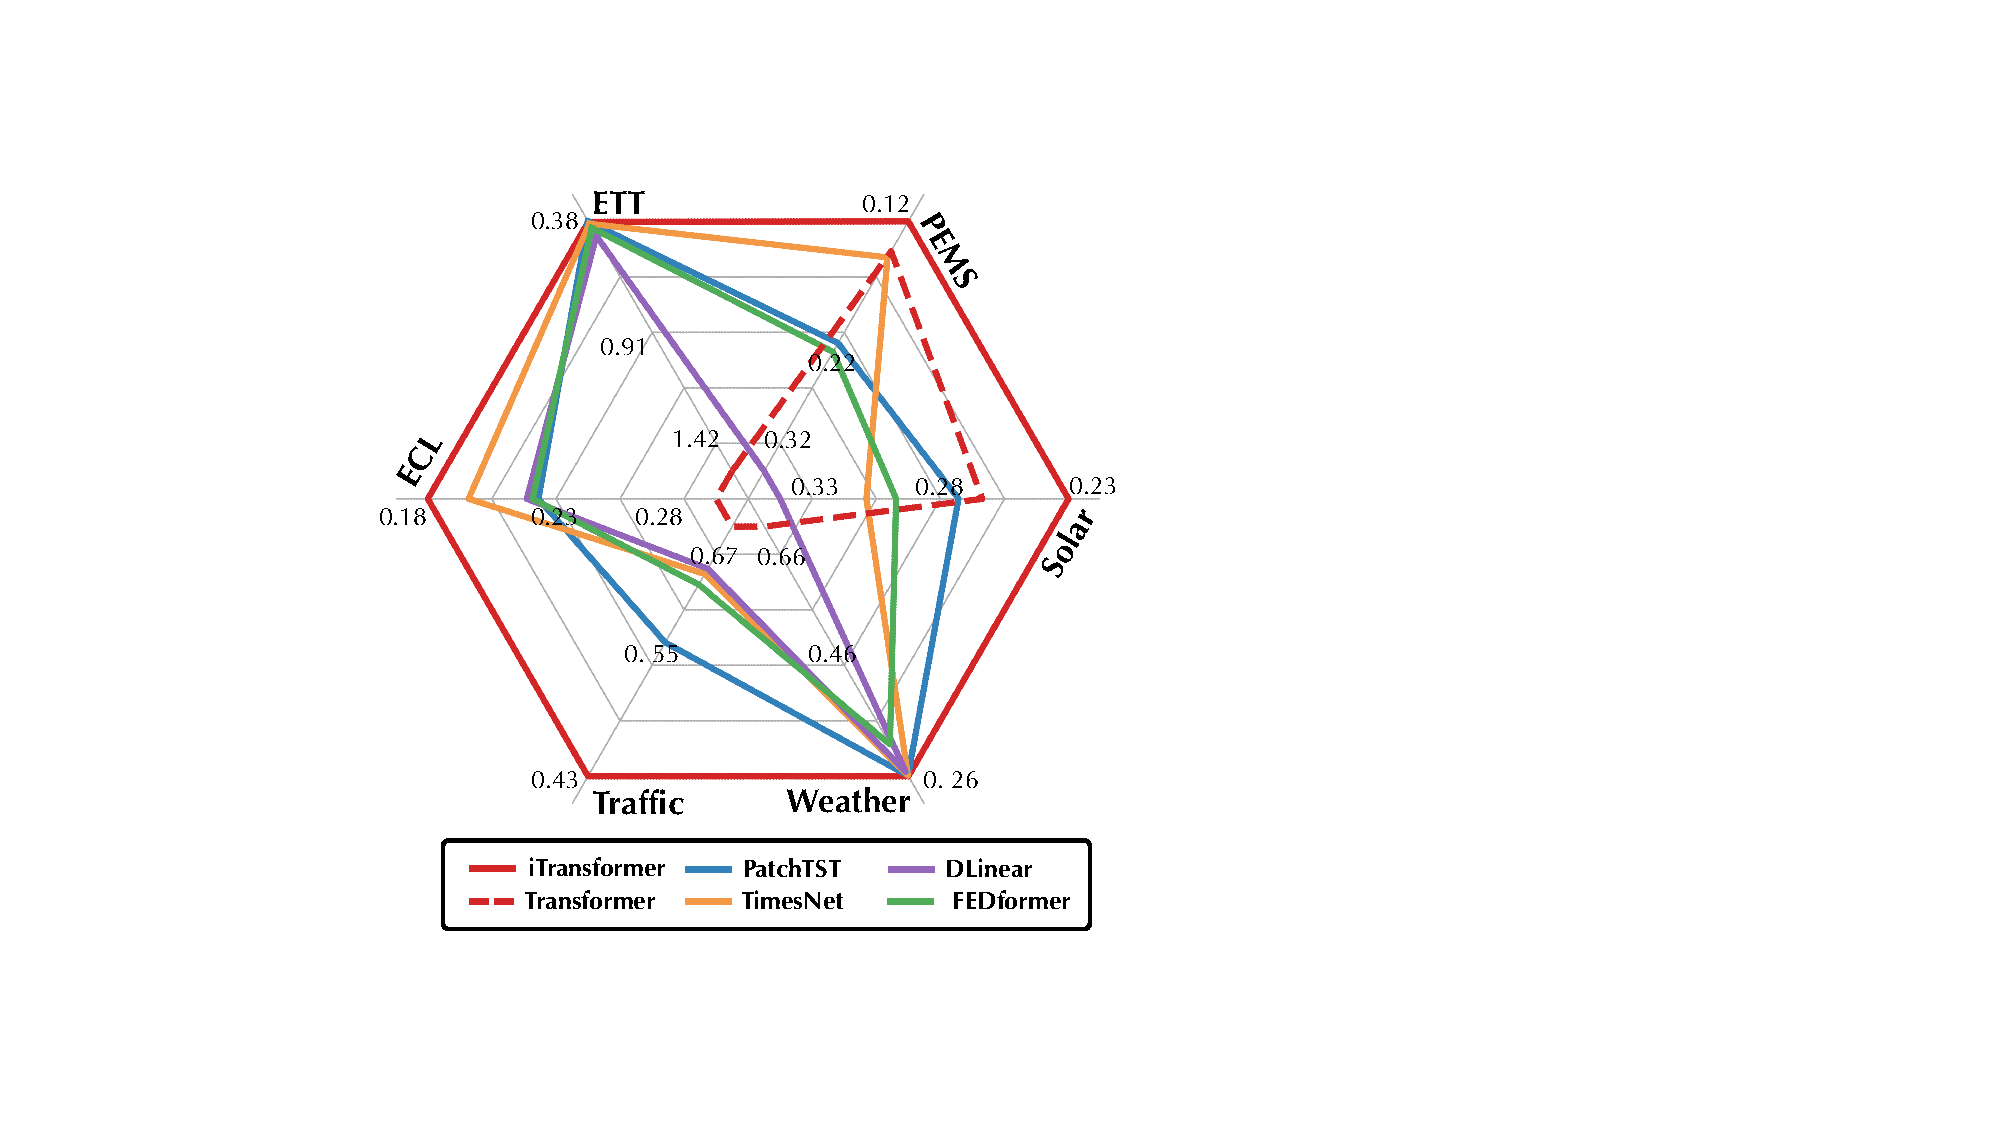
\includegraphics[width=0.5\columnwidth]{pic/radar.pdf}
    % \vspace{-5pt}
    \vspace{-10pt}
    \caption{\small{Performance of iTransformer. Average results (MSE) are reported following TimesNet~\citeyearpar{Timesnet}}.}
    \label{fig:radar}
  \end{center}
  % \vspace{-14pt}
  \vspace{-14pt}
\end{figure}


Transformer~\citep{Transformer} has achieved tremendous success in natural language processing~\citep{brown2020language} and computer vision~\citep{dosovitskiy2020image}, growing into the foundation model that follows the scaling law~\citep{kaplan2020scaling}. Inspired by the immense success in extensive fields, Transformer with strong capabilities of depicting pairwise dependencies and extracting multi-level representations in sequences is emerging in time series forecasting~\citep{Informer, Autoformer, PatchTST}.


However, researchers have recently begun to question the validity of Transformer-based forecasters, which typically embed multiple variates of the same timestamp into indistinguishable channels and apply attention on these \emph{temporal tokens} to capture temporal dependencies. Considering the numerical but less semantic relationship among time points, researchers find that simple linear layers, which can be traced back to statistical forecasters~\citep{box1968some}, have exceeded complicated Transformers on both performance and efficiency~\citep{DLinear, das2023long}. Meanwhile, ensuring the independence of variate and utilizing mutual information is ever more highlighted by recent research that explicitly models multivariate correlations to achieve accurate forecasting~\citep{Crossformer, TSMixer}, but this goal can be hardly achieved without subverting the vanilla Transformer architecture.


Considering the disputes of Transformer-based forecasters, we reflect on why Transformers perform even worse than linear models in time series forecasting while acting predominantly in many other fields. We notice that the existing structure of Transformer-based forecasters may be not suitable for multivariate time series forecasting. As shown on the top of Figure~\ref{fig:motivation}, it is notable that the points of the same time step that basically represent completely different physical meanings recorded by inconsistent measurements are embedded into one token with wiped-out multivariate correlations. And the token formed by a single time step can struggle to reveal beneficial information due to excessively local receptive field and \update{time-unaligned events represented by simultaneous time points}. Besides, while series variations can be greatly influenced by the sequence order, permutation-invariant attention mechanisms are improperly adopted on the temporal dimension~\citep{DLinear}. Consequently, Transformer is weakened to capture essential series representations and portray multivariate correlations, limiting its capacity and generalization ability on diverse time series data.


\update{Concerning the potential risks of embedding multivariate points of a timestamp as a (temporal) token}, we take an \emph{inverted view} on time series and embed the whole time series of each variate independently into a (variate) token, the extreme case of Patching~\citep{PatchTST} that enlarges local receptive field. By inverting, the embedded token aggregates the global representations of series that can be more variate-centric and better leveraged by booming attention mechanisms for multivariate correlating. Meanwhile, the feed-forward network can be proficient enough to learn generalizable representations for distinct variates encoded from arbitrary lookback series and decoded to predict future series.

Based on the above motivations, we believe it is not that Transformer is ineffective for time series forecasting, but rather it is improperly used. In this paper, we revisit the structure of Transformer and advocate \emph{iTransformer} as a fundamental backbone for time series forecasting. Technically, we embed each time series as \emph{variate tokens}, adopt the attention for multivariate correlations, and employ the feed-forward network for series representations. Experimentally, the proposed iTransformer achieves state-of-the-art performance on real-world forecasting benchmarks shown in Figure~\ref{fig:radar} and surprisingly tackles the pain points of  Transformer-based forecasters. Our contributions lie in three aspects:


\begin{figure}[t]
  \begin{center}
    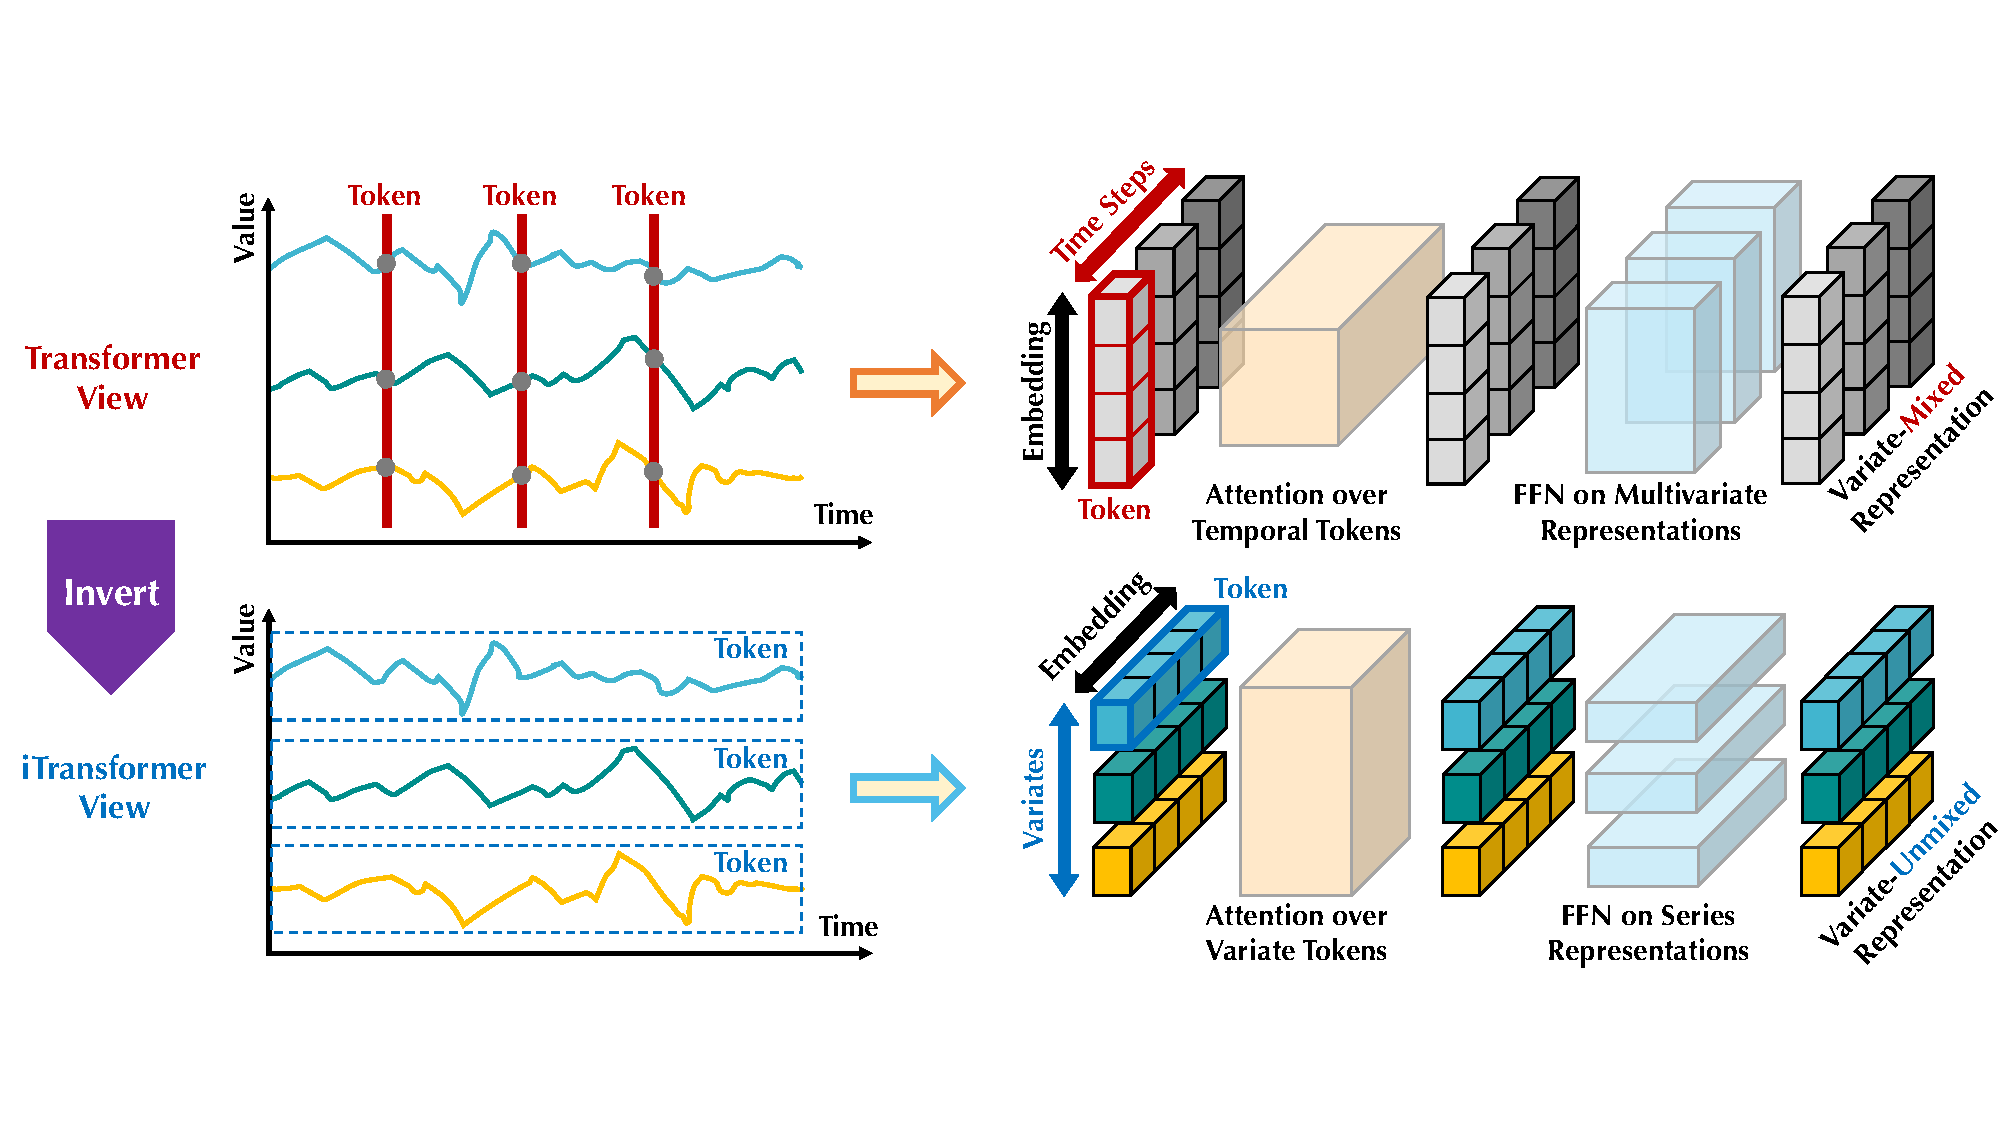
\includegraphics[width=0.95\columnwidth]{pic/motivation.pdf}
    % \vspace{-5pt}
    \vspace{-10pt}
    \caption{\small{\update{Comparison between the vanilla Transformer (top) and the proposed iTransformer (bottom).} Transformer embeds the temporal token, which contains the multivariate representation of each time step. iTransformer embeds each series independently to the variate token, such that the attention module depicts the multivariate correlations and the feed-forward network encodes series representations.}}
    \label{fig:motivation}
  \end{center}
  % \vspace{-14pt}
  \vspace{-14pt}
\end{figure}

\begin{itemize}
  \item We reflect on the architecture of Transformer and refine that the competent capability of native Transformer components on multivariate time series is underexplored.
  \item We propose iTransformer that regards independent time series as tokens to capture multivariate correlations by self-attention and utilize layer normalization and feed-forward network modules to learn better series-global representations for time series forecasting.
  \item Experimentally, iTransformer achieves comprehensive state-of-the-art on real-world benchmarks. We extensively analyze the inverted modules and architecture choices, indicating a promising direction for the future improvement of Transformer-based forecasters.
\end{itemize}

\bibliography{dllab_final_report}
\bibliographystyle{iclr2024_conference}

\vfill

\end{document}
